
\section{Thin Strip Graphs}
\label{sec:thin}


$c$-strip graphs are unit disk graphs such that the centers of the disks belong to
$\{(x,y) : -\infty < x < \infty, 0 < y \leq c\}$. The class is denoted by SG($c$). We
have SG(0) = UIG and SG($\infty$) = UDG. \cite{hayashiThinStripGraphs2017}

\begin{defn}
  Thin strip graphs are defined as TSG $= \bigcap_{c > 0}$ SG($c$).
\end{defn}

\begin{remark}
  SG($0$) $\neq$ TSG. We can construct a $K_{1,3}$ such that we have 3 vertices with the coordinates
  $(1,0)$, $(0,0)$, $(1,0)$ and a last one $(0,\varepsilon)$ with $\varepsilon > 0$ and arbitrarily small
  as seen in Figure \ref{fig:thinK13}.
\end{remark}


% Figure about the K_1,3 construction
\begin{figure}
\centering

\begin{scaletikzpicturetowidth}{\textwidth}
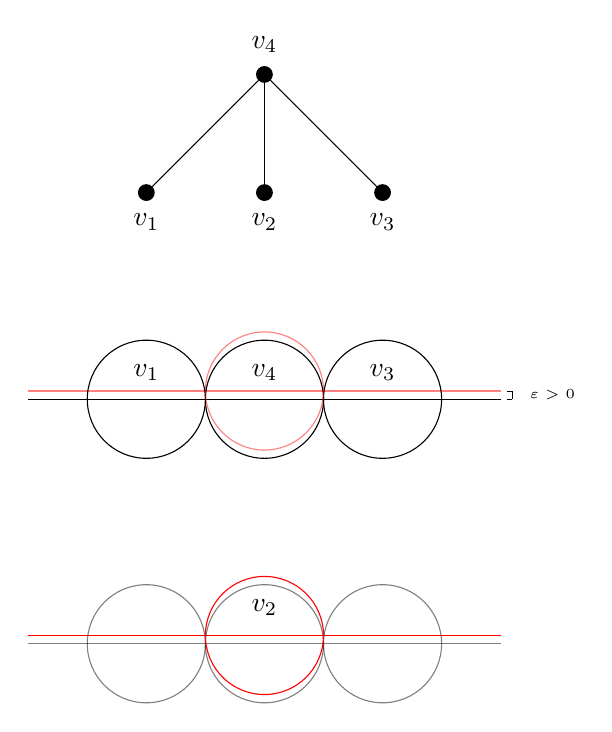
\begin{tikzpicture}[scale=1.5]

\draw (-2,0) -- (2,0);
\draw[red ,opacity = 0.5] (-2,0.07) -- (2,0.07);
\draw  (-1,0) circle [radius=0.5];
\draw[color=black] (-1,0.2265) node {$v_1$};
\draw  (0,0) circle [radius=0.5];
\draw[color=black] (0,0.2265) node {$v_4$};
\draw  (1,0) circle [radius=0.5];
\draw[color=black] (1,0.2265) node {$v_3$};

\draw[red, opacity = 0.5] (0,0.07) circle [radius=0.5];
\draw[color=black] (2.4386,0.0367) node {\tiny $\varepsilon > 0$};

% lines to describe distance (epsilon)
\draw[very thin] (2.1,0.07) -- (2.1,0);
\draw[very thin] (2.05,0.07) -- (2.1,0.07);
\draw[very thin] (2.05,0) -- (2.1,0);

\draw[opacity = 0.5] (-2,-2.07) -- (2,-2.07);
\draw[red] (-2,-2) -- (2,-2);
\draw[opacity = 0.5]  (0,-2.07) circle [radius=0.5];
\draw[opacity = 0.5]  (1,-2.07) circle [radius=0.5];
\draw[opacity = 0.5]  (-1,-2.07) circle [radius=0.5];
\draw[red] (0,-2) circle [radius=0.5];
\draw[color=black] (0,-1.765) node {$v_2$};

\node[draw,circle,inner sep=2pt,fill,label distance=1cm] (v1) at (0,2.75) {};
\draw[color=black] (0,3) node {$v_4$};
\node[draw,circle,inner sep=2pt,fill,label distance=1cm] (v3) at (0,1.75) {};
\draw[color=black] (0,1.5) node {$v_2$};
\node[draw,circle,inner sep=2pt,fill,label distance=1cm] (v2) at (-1,1.75) {};
\draw[color=black] (1,1.5) node {$v_3$};
\node[draw,circle,inner sep=2pt,fill,label distance=1cm] (v4) at (1,1.75) {};
\draw[color=black] (-1,1.5) node {$v_1$};
\draw  (v1) edge (v2);
\draw  (v1) edge (v3);
\draw  (v1) edge (v4);
\end{tikzpicture}
\end{scaletikzpicturetowidth}

\caption{A construction of $K_{1,3}$ with a disk realization, being this graph a TSG.}
\label{fig:thinK13}
\end{figure}

\begin{theorem}
  There is no constant $t$ such that SG($t$) = TSG.
\end{theorem}

Since this class is newly defined we have to characterize it. For this purpose,
some relations have been found between this class and interval graphs.

\subsection{Interval graphs}

\begin{theorem}
  MUIG $\subsetneq$ TSG.
\end{theorem}

We can define a new class of graphs: unfettered unit interval graphs. These graphs
are unit interval graphs where if two intersections touch, we can decide whether
they intersect or not. We denote this class UUIG.

\begin{theorem}
  TSG $\subsetneq$ UUIG.
\end{theorem}


\subsection{Open questions about Thin Strip Graphs}
In this section we state the problems that are being studied for the thesis.

\paragraph{Forbidden subgraphs of Thin Strip Graphs}
  We have proven that MUIG $\subsetneq$ TSG $\subsetneq$ UUIG. Knowing some
  characterizations of MUIG, we can have an approach to this question by
  exploring the already known forbidden subgraphs of MUIG.

  From the results shown in this section, we can say that TSG $\subseteq$ UDG
  $\cap$ UUIG, being UUIG a subclass of co-comparability graphs.

\paragraph{Complexity class for TSG recognition}
  We have shown in section \ref{sec:complex} that some intersection
  geometric problems are in $\exists \mathbb{R}$ (unit disk graph
  recognition problem or the stretchability problem) and we would like to
  know if TSG recognition or even SG($c$) recognition is in NP knowing
  that TSG $\subseteq$ UDG $\cap$ UUIG.

\paragraph{Complexity class of graph problems applied to TSG}
  We have shown in section \ref{sec:complex} that CLIQUE is in $\mathcal{P}$ for
  unit disk graphs. Knowing that TSG $\subseteq$ UDG $\cap$ UUIG we know that CLIQUE
  is also polynomial for TSG. The question is, is there any problem that for the superclasses
  UUIG (and also co-comparability graphs) and UDG whose complexity is reduced for
  TSG or TSG($c$)?

  We can also analyze the domains of $c$ for which some problems are easier. This could
  help us bound the complexity of those problems.
